\parindent=0em
\subsection{Tecnologías en realidad virtual}
\noindent

En el caso de la realidad virtual es necesario tener en cuenta otros factores para una buena experiencia aparte de la posición y orientación del usuario, como por ejemplo, la posición y gestos de las manos o la distancia interpupilar.\\

Primero de todo, hay que tener en cuenta el concepto de DoF (del inglés \textit{Degrees of Freedom}), los DoF hacen referencia a los distintos movimientos o rotaciones que puede tener en cuenta o realizar un elemento. En los dispositivos de realidad virtual se distingue entre 3DoF y 6DoF (figura~\ref{fig:3dofvs6dof}), por ejemplo, en un dispositivo con 3DoF, solo se tiene en cuenta la rotación mientras que si posee 6DoF se tiene en cuenta estas 3 rotaciones y el movimiento del dispositivo en 3 ejes.\\

\begin{figure}[H]
    \centering
    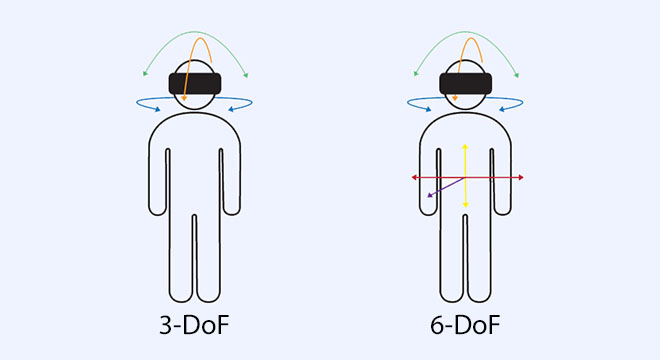
\includegraphics[scale=0.6]{Images/Estado del arte/3dofvs6dof.jpg}
    \caption[Diferenciación entre 3DoF y 6DoF]{Diferenciación entre 3DoF y 6DoF\footnotemark.}
    \label{fig:3dofvs6dof}
\end{figure}
\footnotetext{Fuente: \url{https://virtualspeech.com/blog/degrees-of-freedom-vr}}
%https://virtualspeech.com/blog/degrees-of-freedom-vr

Por otra parte, el \textit{hand tracking} o seguimiento de manos es un proceso mediante el cual se obtiene la posición de las manos y también, los gestos que están realizando como cerrar el puño o agarrar algo, entre otros. Un modelo que se presenta para hacer este seguimiento~\cite{robustHandTracking} habla de la dificultad del proceso debido a la gran cantidad y variación de DoF que pueden tomar las manos. Este modelo se basa en una única cámara de profundidad mediante la cual obtienen imágenes que luego procesan utilizando aprendizaje automático para finalmente poder obtener la posición de las manos y su rotación en tiempo real.\\

Aunque no es obligatorio para un correcto funcionamiento de la realidad virtual que los dispositivos utilicen \textit{hand tracking} (ya que se puede utilizar un par de mandos en su lugar) es un factor que incrementa la inmersión del usuario notablemente, asimismo, no es obligatorio el uso de \textit{eye tracking} o seguimiento de ojos pero puede ser beneficioso para la experiencia. Gracias al \textit{eye tracking} se puede obtener información útil~\cite{eyetrackingVR} como las regiones de interés del espacio 3D y saber en qué momento se ha mirado hacia estas regiones, también, se puede cambiar la información en pantalla basándose en dónde está mirando el usuario o incluso controlar las interfaces virtuales con la mirada.\\

%https://www.vistaoftalmologos.es/realidad-virtual-atencion-los-ojos/#:~:text=En%20los%20juegos%20de%20realidad,confuso%2C%20reconstruye%20una%20imagen%20%C3%BAnica.&text=Para%20continuar%20viendo%20la%20pel%C3%ADcula,la%20convergencia%20y%20la%20acomodaci%C3%B3n.

Cuando se hace uso de un visor de realidad virtual, cada ojo obtiene una imagen ligeramente desplazada en el espacio, lo que provoca que el cerebro reconstruya una imagen única. La distancia interpupilar o IPD (del inglés \textit{Interpupillary Distance}) es otro factor a tener en cuenta a la hora de una experiencia virtual satisfactoria debido al proceso del cerebro de crear dicha imagen única. La IPD es la distancia (normalmente medida en milímetros) entre los centros de los dos ojos (figura~\ref{fig:IPDExample}).

\begin{figure}[H]
    \centering
    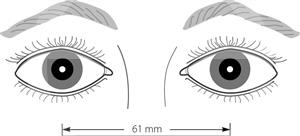
\includegraphics[scale=1]{Images/Estado del arte/IPD.jpg}
    \caption[Medición de la distancia interpupilar]{Medición de la distancia interpupilar\footnotemark.}
    \label{fig:IPDExample}
\end{figure}

\footnotetext{Fuente: \url{https://www.aao.org/image/interpupillary-distance-2}}
Según un estudio realizado con distintas personas haciendo variaciones de la IPD~\cite{IPDTest} en un HMD (del inglés \textit{Head Mounted Display}) o casco de realidad virtual, se llegó a la conclusión de que no había alteraciones a la hora de distinguir los tamaños de los objetos virtuales o afectaciones en la claridad de la visión, en cambio, los usuarios notaron una mayor fatiga con una configuración en el HMD de 50mm y 74mm en la distancia interpupilar en comparación a un valor de la IPD adecuado a su distancia interpupilar anatómica.\\
%https://www.aao.org/image/interpupillary-distance-2

También está relacionado con la visión el concepto de FOV, del inglés \textit{Field Of View}. El FOV hace referencia a la amplitud del campo de visión que ofrece el dispositivo, los seres humanos pueden llegar hasta 180\degree~ gracias a los dos ojos.\\

Para finalizar, respecto a la autonomía de los dispositivos, estos pueden ser inalámbricos o depender de algún cable como fuente de energía. Los dispositivos inalámbricos suelen utilizar pilas o baterías recargables con distintos tiempos de autonomía y en caso de necesitar conectarse a un dispositivo utilizan \textit{bluetooth}. En el caso de no ser inalámbricos los dispositivos suelen conectarse a un ordenador a través de cables HDMI y USB y utilizarlo como fuente de energía.



